\documentclass{article}

\usepackage{fontspec}   %加這個就可以設定字體

\usepackage{lingmacros}
\usepackage{amssymb,amsmath,amsthm, mathtools}
\usepackage{graphicx}
\newtheorem{theorem}{Theorem}
\newtheorem*{theorem*}{Theorem}
\newtheorem*{remark}{Remark}
\usepackage{indentfirst}
\usepackage{tikz}

\begin{document}
\title{Iterative Method For Linear System - Report}
\author{NTU CSIE \& MATH Upstair Looser}
\date{2014/11/24}
\maketitle

\section{Homework Description}
\paragraph{}
In this homework, we are going to use four iterative methods to solve two kind of sparse linear system with different scales. Then compare the performance of each methods. Hoping to get deeper knowledge into the extraordinary iterative linear system method.\\
\indent The four iterative methods are:
\begin{itemize}
\item Gauss-Seidel (GS)
\item PCG with identity matrix as preconditioner
\item PCG with incomplete Cholesky matrix as preconditioner (PCG-IC)
\item Symmetric Gauss-Seidel (Sym-GS)
\end{itemize}

\paragraph{}
There are two type of input linear system in this homework. The first problem is that the matrix is regular and the other is refined at a hole. For each method, we tried three cases with type 1 and 2 cases with type 2. On the other hand, we focus on the following features in the result:
\begin{itemize}
\item Number of iterations
\item Elapsed time
\item Storage
\end{itemize}

\paragraph{}
I'm using Matlab to do the whole calculation in this report. You can find my code and the result .mat file on Google drive. The links are in the reference at the last page of this report\cite{Code}.




% Result
\newpage
\section{Result}

We compare three important features between the four methods we use. The features are: number of iterations, elapsed time, and storage. The result of the first category dataset is as follow:
\begin{figure}[ht!]
\centering
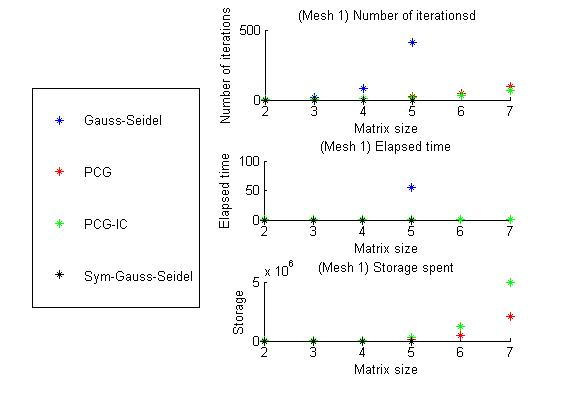
\includegraphics[width=90mm]{mesh1result.jpg}
\caption{Result using mesh 1 dataset}
\label{overflow}
\end{figure}
\begin{figure}[ht!]
\centering
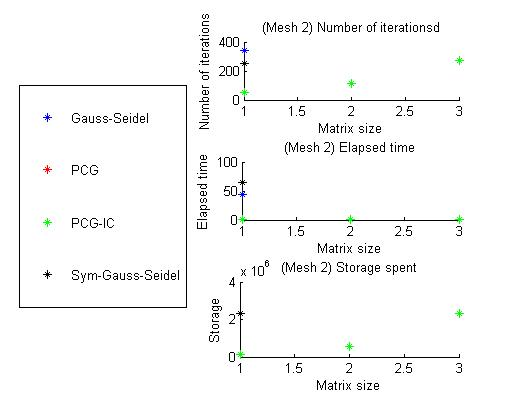
\includegraphics[width=90mm]{mesh2result.jpg}
\caption{Result using mesh 2 dataset}
\label{overflow}
\end{figure}

\newpage
\begin{remark}
The matrices size of the first dataset(mesh1) are 
\begin{table}[h]
\begin{center}
\begin{tabular}{cccccc}

2&3&4&5&6&7\\
\hline
Size = 9 & Size = 49 & Size = 225 & Size 961 & Size = 3969 & Size = 16129\\
\hline
\end{tabular}
\caption{The matrices size of mesh1}
\end{center}
\end{table}

The matrices size of the second dataset(mesh2) are 
\begin{table}[h]
\begin{center}
\begin{tabular}{ccc}

1&2&3\\
\hline
Size = 915 & Size = 3652 & Size = 14586\\
\hline
\end{tabular}
\caption{The matrices size of mesh2}
\end{center}
\end{table}


\end{remark}

% Analysis on nuber of iterations
\subsection{Number of iterations} 
\paragraph{}
First, let's take a look at the number of iterations using four different iterative linear system solving method:
\begin{table}[h]
\begin{center}
\begin{tabular}{lcccccc}
\hline
Method & Size = 9 & Size = 49 & Size = 225 & Size = 961 & Size = 3969 & Size = 16129\\
\hline
GS & 3 & 17 & 85 & 411 & &\\
PCG & 2 & 4 & 10 & 23 & 47 & 95\\
PCG-IC & 1 & 2 & 5 & 12 & 26 & 57\\
Sym-GS & 3 & 14 & 67 & 321 & &\\
\hline
\end{tabular}
\caption{Number of iterations using four iterative methods}
\end{center}
\end{table}


We can easily see that no matter using Gauss-Seidel or symmetric Gauss-Seidel method to solve iterative linear system, the number of iterations will quickly increases.
If we look more deep inside the algorithm of Gauss-Seidel method, we know that the iteration rule of it is as follow:
$$x^{(k+1)} = (D+L)^{-1}Ux^{(k)} + (D+L)^{-1}b$$

\paragraph{}
Recall that the convergence rate of stationary iterative method will be same as the convergence rate of $\|B\|$ to zero, where $B$ is the iteration matrix. Also, the convergence rate of $\|B\|$ to zero is equal to the convergence rate to zero of $B$ 's top eigenvalue $\lambda_{max}$. Using $Matlab$ to calculate the absolute value of the top eigenvalue of the iteration matrices of each size. 
\begin{table}[h]
\begin{center}
\begin{tabular}[c]{lccc}
\hline
 & Size = 9 & Size = 49 & Size = 225 \\
\hline
$\lambda_{max}$ & -0.509587 & -0.854224& -0.961987 \\
\hline
\end{tabular}
\caption{top eigenvalue of the iteration matrices}
\end{center}
\end{table}

\paragraph{}
On the other hand, we know the bond on the error after $k$ iterations of the PCG algorithm:\cite[pp.155-156]{QSS07}
$$\|x^{(k)}-x^*\|_A \leq \frac{2c^k}{1+c^{2k}}\|x^{(0)}-x^*\|_A$$
where
$c = \frac{\sqrt{\kappa(\hat{G})}-1}{\sqrt{\kappa(\hat{G})}+1}$, $\hat{G} = I - G$, $G$ is the iteration matrix
\paragraph{}
This is a tighter upper bound for iteration error than the upper bound given in the homework description.
$$\|x^{(k)}-x^*\|_A \leq 2(\frac{\sqrt{\kappa(\hat{G})}-1}{\sqrt{\kappa(\hat{G})}+1})^k\|x^{(0)}-x^*\|_A$$

\paragraph{}
There are some papers claiming that the rate of convergence of PCG with some specific algorithm in certain cases are quadratic. However, I'm not really understand the proof. A result I found in a paper\cite{CG} seems more reasonable, although it is also a loose upper bound. 

\begin{figure}[h]
\centering
\includegraphics[width=60mm]{convergence_CG_1.png}
\caption{Convergence of Conjugate Gradients (per iteration) as a function of condition number}
\label{overflow}
\end{figure}

\paragraph{}
The estimation is based on condition number. So let's calculate the condition number of iteration matrices of different size. The results are as follow:
\begin{table}[h]
\begin{center}
\begin{tabular}{lcccc}
\hline
Method & Size = 9 & Size = 49 & Size = 225 & Size 961 \\
\hline
$\kappa(A)$ & 9.000 & 37.265 & 150.417 & 603.052\\
\hline
\end{tabular}
\caption{Condition Number of iteration matrices with different size}
\end{center}
\end{table}

\paragraph{}
Consider the iteration matrix with size = 225. Using extrapolation to estimate the convergence rate per iteration is about $0.83$. From Table 2, the convergence rate of same system with Gauss-Seidel method is $0.96$. Thus we can calculate the ratio of the number of iterations between the two methods at the same error level. The result is $\frac{\log0.96}{\log0.83} = 0.2191$, which is closed to the ratio of real number of iterations: $\frac{10}{85} = 0.1176$

\paragraph{}
After comparing the the convergence rate of Gauss-Seidel and PCG, we can learn that the convergence rate of PCG is far more faster than Gauss-Seidel when the iteration will converge.

\paragraph{}
In the end of the discussion about number if iterations, let's consider only using PCG method with preconditioner to be identity matrix and incomplete Cholesky matrix. Since these two methods are relatively fast, I will increase the size of the linear system and observe how the number of iterations change.
\begin{table}[h]
\begin{center}
\begin{tabular}{lcccccc}
\hline
Method & 9 & 49 & 225 & 961 & 3969 & 16129\\
\hline
PCG & 2 & 4 & 10 & 23 & 47 & 95\\
PCG-IC & 2 & 3 & 9 & 17 & 32 & 66\\
\hline
\end{tabular}
\caption{Number of iterations using PCG and PCG-IC iterative methods. The first row is the size of the linear system.}
\end{center}
\end{table}


It's clearly that the number of iterations are smaller when using incomplete Cholesky preconditioner in PCG method. The reason is that the condition number of iteration matrix of PCG-IC is significantly smaller than the usual PCG method. Note that we should consider the condition number of $\hat{G} = I-G$. The condition number of each $\hat{G}$ with different size are listed as follow:

\begin{table}[h]
\begin{center}
\begin{tabular}{lccccc}
\hline
Method & Size = 9 & Size = 49 & Size = 225 & Size 961 & Size = 3969\\
\hline
$\kappa(A)$ & 9.000 & 37.265 & 150.417 & 603.052 & 2413.599\\
$\kappa(P^{-1}A)$ & 1.741 & 6.458 & 24.846 & 100.681 & 403.525\\
\hline
\end{tabular}
\caption{Compare the condition number of A and preconditioned $P^{-1}A$}
\end{center}
\end{table}




% Analysis on Elapsed time
\newpage
\subsection{Elapsed Time}
In the beginning, let's take a look at the elapsed time using four different iterative linear system solving method:
\begin{table}[h]
\begin{center}
\begin{tabular}{lcccccc}
\hline
Method & Size = 9 & Size = 49 & Size = 225 & Size = 961 & Size = 3969 & Size = 16129\\
\hline
GS & 0.0001 & 0.0027 & 0.0795 & 5.9445 & &\\
PCG & 0.0002 & 0.0003 & 0.0009 & 0.0029 & 0.0158 & 0.1079\\
PCG-IC & 0.0004 & 0.0002 & 0.0004 & 0.0019 & 0.0132 & 0.1248\\
Sym-GS & 0.0002 & 0.0036 & 0.1277 & 8.8022 & &\\
\hline
\end{tabular}
\caption{Elapsed time using four iterative methods}
\end{center}
\end{table}


The elapsed time is proportional to the number of iterations multiply an ordered of the iteration matrix size plus some initialization fixed time.
$$t_{elapsed} = n_{iteration} * t_{iteration} + t_{initialization}$$
where, $t_{iteration} = f(n_{matrixSize})$


First, let's consider the difference between the four methods. If we divide the elapse time by the number of iteration, we will get the result as follow:
\begin{table}[h]
\begin{center}
\begin{tabular}{lcccccc}
\hline
Method & Size = 9 & Size = 49 & Size = 225 & Size = 961 & Size = 3969 & Size = 16129\\
\hline
GS & 0.0000 & 0.0002 & 0.0009 & 0.0145 & &\\
PCG & 0.0001 & 0.0001 & 0.0001 & 0.0001 & 0.0003 & 0.0011\\
PCG-IC & 0.0004 & 0.0001 & 0.0001 & 0.0002 & 0.0005 & 0.0022\\
Sym-GS & 0.0001 & 0.0003 & 0.0019 & 0.0274 & &\\
\hline
\end{tabular}
\caption{Elapsed time divided by number of iteration of iterative methods}
\end{center}
\end{table}

We can clearly see that the mean elapsed time per iteration is significantly smaller when using Conjugate methods than using Gauss-Seidel methods. Let's dig into each algorithm and see why PCG is faster.

The following analysis will separated in three parts. The first part is the analysis in Gauss-Seidel and symmetric Gauss-Seidel. The second analysis is about PCG methods with different preconditioners. The last part is the comparison of Gauss-Seidel and PCG methods.

\subsubsection{Gauss-Seidel}
Consider a $n*n$ linear system. In Gauss-Seidel method, there are $n$ vector multiplication for each iteration. Moreover, for symmetric Gauss-Seidel method, there are $2n$ vector multiplication for each iteration. As a result, we can see that the elapsed time of symmetric Gauss-Seidel is about two times to the elapsed time of Gauss-Seidel. 

Since each vector multiplication takes $n$ operations, we can conclude that the complexity of each iteration is $O(n^2)$.
\subsubsection{PCG}
On the other hands, let's consider PCG methods. The whole process involves a matrix inverse operations, and several matrix vector multiplications. We discuss the two main operations respectively. 

The matrix inverse operation is done in preprocessed part of the algorithm which will be only calculated once. For the PCG using identity matrix as preconditioners, inverse operation takes no additional calculation. When using incomplete Cholesky preconditioners, the preprocessing part has two operations: incomplete Cholesky factorization and an inverse operation on a triangular matrix. The complexity of Cholesky factorization is $n^3/3$. Also, the complexity of triangular matrix inverse operation is about $n^3/3$. As a result, the complexity of the preprocessing part of the PCG using incomplete Cholesky preconditioners is $O(n^3)$.

As to the matrix vector multiplications part, the complexity is only $O(n^2)$

\subsubsection{Gauss-Seidel and PCG}
From the above analysis, we can see that both Gauss-Seidel and PCG algorithm has $O(n^2)$ complexity in each iteration. PCG with incomplete Cholesky preconditioners are expensive during preprocessing since it has to factorize a matrix in $O(n^2)$ and inverse a triangular matrix. 

Let's study the result, it shows that the cost of each iteration is more expensive when using Gauss-Seidel algorithm. However, the analysis tells us that the complexity of both algorith are in the same order, $O(n^2)$. When using Gauss-Seidel algorithm, it performs $n$ vector multiplications, while in PCG algorithm, it performs a product of matrix and vector. Both $n$ vector multiplications and product of matrix and vector take about $O(n^2)$ operations. Why is that they have the same complexity order but result in very different result?

The reason is that the $n$ vector multiplications performed in Gauss-Seidel is not parallel, it's sequential! As a result, in each iteration, it needs to complete the $O(n^2)$ operations sequentially, while the product of matrix and vector in PCG can be calculated in parallel. We compare the elapsed time used in a product of matrix and vector with two different methods: the first method sequentially calculates the vector multiplications for $n$ times, and the other is to calculate the result using the matrix vector multiplication operation directly in Matlab. The results are as follow:

\begin{table}[h]
\begin{center}
\begin{tabular}{lcccccc}
\hline
Method & Size = 9 & Size = 49 & Size = 225 & Size = 961 & Size = 3969 & Size = 16129\\
\hline
Sequential & 0.0000 & 0.0002 & 0.0009 & 0.0134 & 0.2693 & 7.0105\\
Direct & 0.0000 & 0.0000 & 0.0001 & 0.0005 & 0.0081 & 0.1793\\
\hline
\end{tabular}
\caption{Elapsed time calculating product of matrix and vector with different approach}
\end{center}
\end{table}

We can easily see that when calculating the product of matrix and vector sequentially through every row takes more time than simply using the direct matrix vector multiplication function in Matlab.Especially when the system size grows up, the difference is much more bigger.

Note that the matrices we used in this experiment is the linear system matrices in the homework problem. So they are all sparse matrices. For a non-sparse matrix, the result will be more dramatically because of more arithmetic operations. 



% Analysis on Storage
\subsection{Storage}
The storages used in different size of linear system with each iterative method are listed as follow:


\begin{table}[h]
\begin{center}
\begin{tabular}{lcccccc}
\hline
Method & Size = 9 & Size = 49 & Size = 225 & Size = 961 & Size = 3969 & Size = 16129\\
\hline
GS & 752 & 4656 & 22448 & 97968 & &\\
GS(full) & 792 & 19992 & 408600 & 7403544 & &\\
PCG & 968 & 5832 & 27848 & 121032 & 504008 & 2056392\\
PCG-IC & 2104 & 13016 & 62840 & 286392 & 1204152 & 4928824\\
Sym-GS & 792 & 4656 & 22448 & 97968 & &\\
Sym-GS(full) & 792 & 19992 & 408600 & 7403544 & &\\
\hline
\end{tabular}
\caption{Storage using four iterative methods}
\end{center}
\end{table}

From the above table, we can see that the storage used in PCG is a little greater than Gauss-Seidel algorithm using sparse data structure. However, when Gauss-Seidel algorithms choose to use full matrix data structure in order to accelerate elapsed time, the storage be dramatically increase and surpass the storage used in PCG algorithm. 

For PCG algorithm using different preconditioners. When using incomplete Cholesky preconditioners, there are additional storage for inverse matrces, while using identity matrices as preconditioners don't have to allocate additional space.

\section{Reordering}

Our results when using reordering are not significantly improved. We believe that it is stemmed from the core of the algorithm. In the following discussion, we first compare the convergence rate before and after the reordering process. Then talk a little about storage issues. At last, we dig into the core of Gauss-Seidel algorithm and PCG algorithm respectively to see how reordering affects the elapsed time.

\subsection{Convergence Rate}
Let's consider the convergence rate before and after the reordering process. We simply calculate the condition number of both original iteration matrix and reordered iteration matrix. The results were the same! Which means that the convergence rate will be the same after reordering the iteration matrix. This analysis result gives a clear answer to why we got a similar results on whether using reordering or not.

\subsection{Storage}
Since the main process in both algorithm will be the same after reordering the iteration matrix, the additional storage will only happens in the reordered result. That is the vector the stores the reordered pattern. Thus, the storage before and after the reordering process will not grow significantly.


\subsection{Elapsed Time in Gauss-Seidel Algorithm}
For Gauss-Seidel algorithm, the iteration is somehow like a backward substitution in LU factorization. However, the algorithm doesn't have the factorization process and doesn't create new fill-in. As a result, it's clearly that when using reordering, the the number of arithmetical operations will nearly be the same. The performance will not improved in the elapsed time of iterations. 


\subsection{Elapsed Time in PCG Algorithm}
The main arithmetical operations in PCG algorithm has three parts. The first part is matrix vector multiplications, which will not be greatly affected by the reordered result. The second part is solving the preconditioned linear system. Whether we calculate the inverse matrix in advance or using backward substitution in each iteration, the most important factor who affect the elapsed time is the number of non-zero elements in iteration matrix. The followings are the number of non-zero elements before and after the reordering process.

\begin{table}[h]
\begin{center}
\begin{tabular}{lcccccc}
\hline
Method & Size = 9 & Size = 49 & Size = 225 & Size = 961 & Size = 3969 & Size = 16129\\
\hline
Before & 45 & 341 & 1749 & 7829 & 33045 & 135701\\
After & 41 & 325 & 1745 & 7965 & 33865 & 139529\\
\hline
\end{tabular}
\caption{Number of non-zero elements before and after the reordering process}
\end{center}
\end{table}

We can see that the number of non-zero elements in iteration matrix before and after the reordering process is very close. When the size of the system grows larger, the number of non-zero elements even are smaller without reordering. From this observation, we can conclude that the reordering process doesn't affect the elapsed time of the algorithm much.

Last but not the least, the elapsed time for incomplete Cholesky factorization is also concerned. However, in this homework, the elapsed time for incomplete Cholesky factorization is at $10^{-3}$ level, which is at noise level and doesn't affect the result much.

\paragraph{}
Conclude the above statements and analysis, we found out that the reordering process doesn't affect the result of the dataset in this homework.

\section{Problem 4}

Consider SIM
$$Mx^{(k+1)}=Nx^{(k)} + b$$

or
$$x^{(k+1)} = M^{-1}Nx^{(k)} + M^{-1}b$$

Show that
$$x^{(k+1)} = x^{(k)} + M^{-1}r^{(k)}$$

and therefore the step the SIM takes is
$$x^{(k+1)}-x^{(k)}=M^{-1}r^{(k)}$$
$sol:$

By the definition of residual we know that
$$r^{(k)} = b - Ax^{(k)}$$

and the relationship between $M$,$N$,and$A$
$$A = M-N$$


replace $N$ with $M-A$ we got
$$x^{(k+1)} = M^{-1}(M-A)x^{(k)} + M^{-1}b$$
$$x^{(k+1)} = x^{(k)} - M^{-1}Ax^{(k)} + M^{-1}b$$
$$x^{(k+1)}-x^{(k)}=M^{-1}(b-x^{(k)})$$

Finally, we got
$$x^{(k+1)}-x^{(k)}=M^{-1}r^{(k)}$$

\section{Remarks}

During the whole experiment, the results had been modified various of time because of the design and implementation of each algorithms. In this section, we list some problem we had encountered and the improvement we have done.

\subsection{Convergence}
The number of iterations is very different in Gauss-Seidel algorithm and PCG algorithms. This is the result of different rate of convergence. We can easily understand the reason is that in PCG methods, each iteration gives the best guess in current state. In other words, PCG methods minimize the energy norm of the residual in current {\it Krylov subspace}. However, when we started to analyse the rate of convergence of PCG algorithms, we found it difficult to give an accurate estimation. The rate of convergence seems to lie between quadratic and linear convergence. Moreover, the upper bound given by the textbook or some other references are too loose.

Finally, we gave up seeking for a tight bound for the convergence rate of PCG methods. Instead, we compare the condition number of different iteration matrices. And showed that the smaller the condition number of the iteration matrix is, the less iterations of convergence are needed. Also, we found a paper discussed PCG method's rate of convergence.\cite{CG}


\subsection{Sparse of Full}
In the first version of our algorithms implementation, the result of Gauss-Seidel algorithm is very bad. The elapsed time is much greater than the time used in PCG methods. 

After a discussion with prof.Wang, we found out that the vector multiplications in in each iteration do not utilize the benefit of sparse structure. In contrast, the sparse structure makes the vectorized multiplications more expensive because of the row extraction operations. As a result, sparse structure doesn't improve the performance, and even makes the result worse.

Then we change the data structure of linear system matrix from sparse structure to full structure. Although the amount of storage significantly increased, the elapsed time was improved. This is a trade off between time and space.

\subsection{Vector Multiplication is Expensive}
After changing the matrix data structure, there's still exists a large gap between the elapsed time per iteration on Gauss-Seidel method and PCG method. Just as the reason mentioned above, the cost of $n$ vector multiplications are much greater than the cost of product between matrix and vector. 

\subsection{Inverse Operations}
In the classroom log on 11/26, TA said that it's abandoned to use Matlab functions to calculate inverse matrix or solve linear system problem in PCG methods. When using incomplete Cholesky preconditioners, the inverse process involves two backward substitutions. However, the linear system in this homework is sparse. As a result, direct backward substitution will have poor performance. To solve this problem, the algorithm needs to utilize sparse structure. Because we are not familiar with sparse algorithm, so we still use Matlab built-in function to solve the inverse problem.



\newpage
% Reference
\renewcommand\refname{Reference}
\bibliographystyle{plain}
\bibliography{Thesis}

\end{document}
